\documentclass[1p]{elsarticle_modified}
%\bibliographystyle{elsarticle-num}

%\usepackage[colorlinks]{hyperref}
%\usepackage{abbrmath_seonhwa} %\Abb, \Ascr, \Acal ,\Abf, \Afrak
\usepackage{amsfonts}
\usepackage{amssymb}
\usepackage{amsmath}
\usepackage{amsthm}
\usepackage{scalefnt}
\usepackage{amsbsy}
\usepackage{kotex}
\usepackage{caption}
\usepackage{subfig}
\usepackage{color}
\usepackage{graphicx}
\usepackage{xcolor} %% white, black, red, green, blue, cyan, magenta, yellow
\usepackage{float}
\usepackage{setspace}
\usepackage{hyperref}

\usepackage{tikz}
\usetikzlibrary{arrows}

\usepackage{multirow}
\usepackage{array} % fixed length table
\usepackage{hhline}

%%%%%%%%%%%%%%%%%%%%%
\makeatletter
\renewcommand*\env@matrix[1][\arraystretch]{%
	\edef\arraystretch{#1}%
	\hskip -\arraycolsep
	\let\@ifnextchar\new@ifnextchar
	\array{*\c@MaxMatrixCols c}}
\makeatother %https://tex.stackexchange.com/questions/14071/how-can-i-increase-the-line-spacing-in-a-matrix
%%%%%%%%%%%%%%%

\usepackage[normalem]{ulem}

\newcommand{\msout}[1]{\ifmmode\text{\sout{\ensuremath{#1}}}\else\sout{#1}\fi}
%SOURCE: \msout is \stkout macro in https://tex.stackexchange.com/questions/20609/strikeout-in-math-mode

\newcommand{\cancel}[1]{
	\ifmmode
	{\color{red}\msout{#1}}
	\else
	{\color{red}\sout{#1}}
	\fi
}

\newcommand{\add}[1]{
	{\color{blue}\uwave{#1}}
}

\newcommand{\replace}[2]{
	\ifmmode
	{\color{red}\msout{#1}}{\color{blue}\uwave{#2}}
	\else
	{\color{red}\sout{#1}}{\color{blue}\uwave{#2}}
	\fi
}

\newcommand{\Sol}{\mathcal{S}} %segment
\newcommand{\D}{D} %diagram
\newcommand{\A}{\mathcal{A}} %arc


%%%%%%%%%%%%%%%%%%%%%%%%%%%%%5 test

\def\sl{\operatorname{\textup{SL}}(2,\Cbb)}
\def\psl{\operatorname{\textup{PSL}}(2,\Cbb)}
\def\quan{\mkern 1mu \triangleright \mkern 1mu}

\theoremstyle{definition}
\newtheorem{thm}{Theorem}[section]
\newtheorem{prop}[thm]{Proposition}
\newtheorem{lem}[thm]{Lemma}
\newtheorem{ques}[thm]{Question}
\newtheorem{cor}[thm]{Corollary}
\newtheorem{defn}[thm]{Definition}
\newtheorem{exam}[thm]{Example}
\newtheorem{rmk}[thm]{Remark}
\newtheorem{alg}[thm]{Algorithm}

\newcommand{\I}{\sqrt{-1}}
\begin{document}

%\begin{frontmatter}
%
%\title{Boundary parabolic representations of knots up to 8 crossings}
%
%%% Group authors per affiliation:
%\author{Yunhi Cho} 
%\address{Department of Mathematics, University of Seoul, Seoul, Korea}
%\ead{yhcho@uos.ac.kr}
%
%
%\author{Seonhwa Kim} %\fnref{s_kim}}
%\address{Center for Geometry and Physics, Institute for Basic Science, Pohang, 37673, Korea}
%\ead{ryeona17@ibs.re.kr}
%
%\author{Hyuk Kim}
%\address{Department of Mathematical Sciences, Seoul National University, Seoul 08826, Korea}
%\ead{hyukkim@snu.ac.kr}
%
%\author{Seokbeom Yoon}
%\address{Department of Mathematical Sciences, Seoul National University, Seoul, 08826,  Korea}
%\ead{sbyoon15@snu.ac.kr}
%
%\begin{abstract}
%We find all boundary parabolic representation of knots up to 8 crossings.
%
%\end{abstract}
%\begin{keyword}
%    \MSC[2010] 57M25 
%\end{keyword}
%
%\end{frontmatter}

%\linenumbers
%\tableofcontents
%
\newcommand\colored[1]{\textcolor{white}{\rule[-0.35ex]{0.8em}{1.4ex}}\kern-0.8em\color{red} #1}%
%\newcommand\colored[1]{\textcolor{white}{ #1}\kern-2.17ex	\textcolor{white}{ #1}\kern-1.81ex	\textcolor{white}{ #1}\kern-2.15ex\color{red}#1	}

{\Large $\underline{12n_{0753}~(K12n_{0753})}$}

\setlength{\tabcolsep}{10pt}
\renewcommand{\arraystretch}{1.6}
\vspace{1cm}\begin{tabular}{m{100pt}>{\centering\arraybackslash}m{274pt}}
\multirow{5}{120pt}{
	\centering
	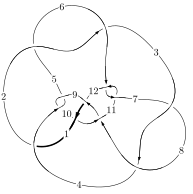
\includegraphics[width=112pt]{../../../GIT/diagram.site/Diagrams/png/2842_12n_0753.png}\\
\ \ \ A knot diagram\footnotemark}&
\allowdisplaybreaks
\textbf{Linearized knot diagam} \\
\cline{2-2}
 &
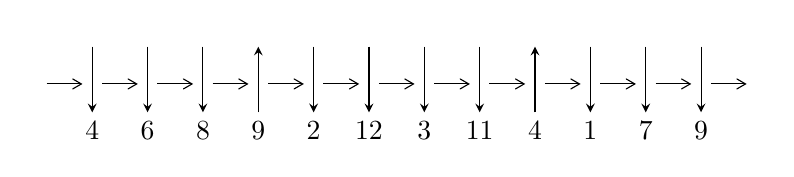
\begin{tikzpicture}[x=20pt, y=17pt]
	% nodes
	\node (C0) at (0, 0) {};
	\node (C1) at (1, 0) {};
	\node (C1U) at (1, +1) {};
	\node (C1D) at (1, -1) {4};

	\node (C2) at (2, 0) {};
	\node (C2U) at (2, +1) {};
	\node (C2D) at (2, -1) {6};

	\node (C3) at (3, 0) {};
	\node (C3U) at (3, +1) {};
	\node (C3D) at (3, -1) {8};

	\node (C4) at (4, 0) {};
	\node (C4U) at (4, +1) {};
	\node (C4D) at (4, -1) {9};

	\node (C5) at (5, 0) {};
	\node (C5U) at (5, +1) {};
	\node (C5D) at (5, -1) {2};

	\node (C6) at (6, 0) {};
	\node (C6U) at (6, +1) {};
	\node (C6D) at (6, -1) {12};

	\node (C7) at (7, 0) {};
	\node (C7U) at (7, +1) {};
	\node (C7D) at (7, -1) {3};

	\node (C8) at (8, 0) {};
	\node (C8U) at (8, +1) {};
	\node (C8D) at (8, -1) {11};

	\node (C9) at (9, 0) {};
	\node (C9U) at (9, +1) {};
	\node (C9D) at (9, -1) {4};

	\node (C10) at (10, 0) {};
	\node (C10U) at (10, +1) {};
	\node (C10D) at (10, -1) {1};

	\node (C11) at (11, 0) {};
	\node (C11U) at (11, +1) {};
	\node (C11D) at (11, -1) {7};

	\node (C12) at (12, 0) {};
	\node (C12U) at (12, +1) {};
	\node (C12D) at (12, -1) {9};
	\node (C13) at (13, 0) {};

	% arrows
	\draw[->,>={angle 60}]
	(C0) edge (C1) (C1) edge (C2) (C2) edge (C3) (C3) edge (C4) (C4) edge (C5) (C5) edge (C6) (C6) edge (C7) (C7) edge (C8) (C8) edge (C9) (C9) edge (C10) (C10) edge (C11) (C11) edge (C12) (C12) edge (C13) ;	\draw[->,>=stealth]
	(C1U) edge (C1D) (C2U) edge (C2D) (C3U) edge (C3D) (C4D) edge (C4U) (C5U) edge (C5D) (C6U) edge (C6D) (C7U) edge (C7D) (C8U) edge (C8D) (C9D) edge (C9U) (C10U) edge (C10D) (C11U) edge (C11D) (C12U) edge (C12D) ;
	\end{tikzpicture} \\
\hhline{~~} \\& 
\textbf{Solving Sequence} \\ \cline{2-2} 
 &
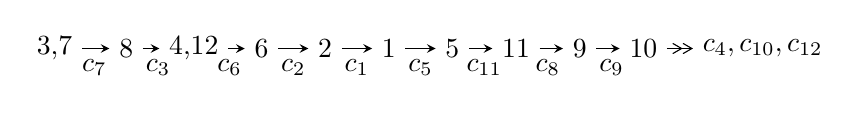
\begin{tikzpicture}[x=23pt, y=7pt]
	% node
	\node (A0) at (-1/8, 0) {3,7};
	\node (A1) at (1, 0) {8};
	\node (A2) at (33/16, 0) {4,12};
	\node (A3) at (25/8, 0) {6};
	\node (A4) at (33/8, 0) {2};
	\node (A5) at (41/8, 0) {1};
	\node (A6) at (49/8, 0) {5};
	\node (A7) at (57/8, 0) {11};
	\node (A8) at (65/8, 0) {9};
	\node (A9) at (73/8, 0) {10};
	\node (C1) at (1/2, -1) {$c_{7}$};
	\node (C2) at (3/2, -1) {$c_{3}$};
	\node (C3) at (21/8, -1) {$c_{6}$};
	\node (C4) at (29/8, -1) {$c_{2}$};
	\node (C5) at (37/8, -1) {$c_{1}$};
	\node (C6) at (45/8, -1) {$c_{5}$};
	\node (C7) at (53/8, -1) {$c_{11}$};
	\node (C8) at (61/8, -1) {$c_{8}$};
	\node (C9) at (69/8, -1) {$c_{9}$};
	\node (A10) at (11, 0) {$c_{4},c_{10},c_{12}$};

	% edge
	\draw[->,>=stealth]	
	(A0) edge (A1) (A1) edge (A2) (A2) edge (A3) (A3) edge (A4) (A4) edge (A5) (A5) edge (A6) (A6) edge (A7) (A7) edge (A8) (A8) edge (A9) ;
	\draw[->>,>={angle 60}]	
	(A9) edge (A10);
\end{tikzpicture} \\ 

\end{tabular} \\

\footnotetext{
The image of knot diagram is generated by the software ``\textbf{Draw programme}" developed by Andrew Bartholomew(\url{http://www.layer8.co.uk/maths/draw/index.htm\#Running-draw}), where we modified some parts for our purpose(\url{https://github.com/CATsTAILs/LinksPainter}).
}\phantom \\ \newline 
\centering \textbf{Ideals for irreducible components\footnotemark of $X_{\text{par}}$} 
 
\begin{align*}
I^u_{1}&=\langle 
-1.36970\times10^{192} u^{71}+1.13541\times10^{192} u^{70}+\cdots+8.77978\times10^{191} b-2.52244\times10^{193},\\
\phantom{I^u_{1}}&\phantom{= \langle  }-2.76575\times10^{194} u^{71}+7.05669\times10^{194} u^{70}+\cdots+6.36534\times10^{194} a-1.06301\times10^{196},\\
\phantom{I^u_{1}}&\phantom{= \langle  }2 u^{72}-3 u^{71}+\cdots-314 u-29\rangle \\
I^u_{2}&=\langle 
1624226 u^{15}+189101 u^{14}+\cdots+2048967 b-3069244,\\
\phantom{I^u_{2}}&\phantom{= \langle  }1675780 u^{15}-2140649 u^{14}+\cdots+2048967 a+298066,\;u^{16}- u^{15}+\cdots- u+1\rangle \\
I^u_{3}&=\langle 
b+a+2,\;a^2+3 a+3,\;u+1\rangle \\
I^u_{4}&=\langle 
b-1,\;a,\;u+1\rangle \\
I^u_{5}&=\langle 
b-1,\;a-3,\;2 u-1\rangle \\
\\
\end{align*}
\raggedright * 5 irreducible components of $\dim_{\mathbb{C}}=0$, with total 92 representations.\\
\footnotetext{All coefficients of polynomials are rational numbers. But the coefficients are sometimes approximated in decimal forms when there is not enough margin.}
\newpage
\renewcommand{\arraystretch}{1}
\centering \section*{I. $I^u_{1}= \langle -1.37\times10^{192} u^{71}+1.14\times10^{192} u^{70}+\cdots+8.78\times10^{191} b-2.52\times10^{193},\;-2.77\times10^{194} u^{71}+7.06\times10^{194} u^{70}+\cdots+6.37\times10^{194} a-1.06\times10^{196},\;2 u^{72}-3 u^{71}+\cdots-314 u-29 \rangle$}
\flushleft \textbf{(i) Arc colorings}\\
\begin{tabular}{m{7pt} m{180pt} m{7pt} m{180pt} }
\flushright $a_{3}=$&$\begin{pmatrix}0\\u\end{pmatrix}$ \\
\flushright $a_{7}=$&$\begin{pmatrix}1\\0\end{pmatrix}$ \\
\flushright $a_{8}=$&$\begin{pmatrix}1\\u^2\end{pmatrix}$ \\
\flushright $a_{4}=$&$\begin{pmatrix}- u\\- u^3+u\end{pmatrix}$ \\
\flushright $a_{12}=$&$\begin{pmatrix}0.434501 u^{71}-1.10861 u^{70}+\cdots+347.297 u+16.7000\\1.56006 u^{71}-1.29321 u^{70}+\cdots+356.879 u+28.7301\end{pmatrix}$ \\
\flushright $a_{6}=$&$\begin{pmatrix}0.0355412 u^{71}+0.176136 u^{70}+\cdots-11.6952 u-6.02177\\3.01683 u^{71}-1.28760 u^{70}+\cdots+385.689 u+33.1010\end{pmatrix}$ \\
\flushright $a_{2}=$&$\begin{pmatrix}1.01568 u^{71}-0.393073 u^{70}+\cdots+193.878 u+14.0114\\-2.66963 u^{71}+1.21209 u^{70}+\cdots-462.369 u-40.0424\end{pmatrix}$ \\
\flushright $a_{1}=$&$\begin{pmatrix}-1.45544 u^{71}+1.03210 u^{70}+\cdots-279.270 u-26.0870\\-2.04836 u^{71}+1.02912 u^{70}+\cdots-383.249 u-33.0258\end{pmatrix}$ \\
\flushright $a_{5}=$&$\begin{pmatrix}1.33808 u^{71}-0.482894 u^{70}+\cdots+103.747 u+5.16521\\0.454400 u^{71}+0.395730 u^{70}+\cdots-29.3983 u-1.94875\end{pmatrix}$ \\
\flushright $a_{11}=$&$\begin{pmatrix}1.99456 u^{71}-2.40182 u^{70}+\cdots+704.175 u+45.4301\\1.56006 u^{71}-1.29321 u^{70}+\cdots+356.879 u+28.7301\end{pmatrix}$ \\
\flushright $a_{9}=$&$\begin{pmatrix}-1.11558 u^{71}+1.08287 u^{70}+\cdots-292.574 u-16.4833\\0.445103 u^{71}-0.585548 u^{70}+\cdots+202.903 u+17.1718\end{pmatrix}$ \\
\flushright $a_{10}=$&$\begin{pmatrix}-2.49602 u^{71}+1.67951 u^{70}+\cdots-453.851 u-30.5168\\0.204348 u^{71}-0.282806 u^{70}+\cdots+112.741 u+9.83185\end{pmatrix}$\\&\end{tabular}
\flushleft \textbf{(ii) Obstruction class $= -1$}\\~\\
\flushleft \textbf{(iii) Cusp Shapes $= -10.8009 u^{71}+8.28607 u^{70}+\cdots-2650.54 u-220.978$}\\~\\
\newpage\renewcommand{\arraystretch}{1}
\flushleft \textbf{(iv) u-Polynomials at the component}\newline \\
\begin{tabular}{m{50pt}|m{274pt}}
Crossings & \hspace{64pt}u-Polynomials at each crossing \\
\hline $$\begin{aligned}c_{1}\end{aligned}$$&$\begin{aligned}
&2(2 u^{72}-7 u^{71}+\cdots+3152 u+248)
\end{aligned}$\\
\hline $$\begin{aligned}c_{2},c_{5}\end{aligned}$$&$\begin{aligned}
&u^{72}+2 u^{71}+\cdots+3215 u+491
\end{aligned}$\\
\hline $$\begin{aligned}c_{3},c_{7}\end{aligned}$$&$\begin{aligned}
&2(2 u^{72}-3 u^{71}+\cdots-314 u-29)
\end{aligned}$\\
\hline $$\begin{aligned}c_{4},c_{9}\end{aligned}$$&$\begin{aligned}
&2(2 u^{72}+3 u^{71}+\cdots-3289 u+373)
\end{aligned}$\\
\hline $$\begin{aligned}c_{6},c_{11}\end{aligned}$$&$\begin{aligned}
&u^{72}+2 u^{71}+\cdots-32 u-13
\end{aligned}$\\
\hline $$\begin{aligned}c_{8}\end{aligned}$$&$\begin{aligned}
&u^{72}-9 u^{71}+\cdots-34 u-16
\end{aligned}$\\
\hline $$\begin{aligned}c_{10}\end{aligned}$$&$\begin{aligned}
&u^{72}- u^{71}+\cdots-868 u+172
\end{aligned}$\\
\hline $$\begin{aligned}c_{12}\end{aligned}$$&$\begin{aligned}
&4(4 u^{72}+7 u^{71}+\cdots+3105391 u-546509)
\end{aligned}$\\
\hline
\end{tabular}\\~\\
\newpage\renewcommand{\arraystretch}{1}
\flushleft \textbf{(v) Riley Polynomials at the component}\newline \\
\begin{tabular}{m{50pt}|m{274pt}}
Crossings & \hspace{64pt}Riley Polynomials at each crossing \\
\hline $$\begin{aligned}c_{1}\end{aligned}$$&$\begin{aligned}
&4(4 y^{72}+315 y^{71}+\cdots+1.07828\times10^{7} y+61504)
\end{aligned}$\\
\hline $$\begin{aligned}c_{2},c_{5}\end{aligned}$$&$\begin{aligned}
&y^{72}-34 y^{71}+\cdots-7263547 y+241081
\end{aligned}$\\
\hline $$\begin{aligned}c_{3},c_{7}\end{aligned}$$&$\begin{aligned}
&4(4 y^{72}-149 y^{71}+\cdots-158162 y+841)
\end{aligned}$\\
\hline $$\begin{aligned}c_{4},c_{9}\end{aligned}$$&$\begin{aligned}
&4(4 y^{72}-273 y^{71}+\cdots-1.06512\times10^{7} y+139129)
\end{aligned}$\\
\hline $$\begin{aligned}c_{6},c_{11}\end{aligned}$$&$\begin{aligned}
&y^{72}+40 y^{71}+\cdots+1758 y+169
\end{aligned}$\\
\hline $$\begin{aligned}c_{8}\end{aligned}$$&$\begin{aligned}
&y^{72}+13 y^{71}+\cdots-21636 y+256
\end{aligned}$\\
\hline $$\begin{aligned}c_{10}\end{aligned}$$&$\begin{aligned}
&y^{72}+71 y^{71}+\cdots+1106584 y+29584
\end{aligned}$\\
\hline $$\begin{aligned}c_{12}\end{aligned}$$&$\begin{aligned}
&16(16 y^{72}+383 y^{71}+\cdots-2.25832\times10^{13} y+2.98672\times10^{11})
\end{aligned}$\\
\hline
\end{tabular}\\~\\
\newpage\flushleft \textbf{(vi) Complex Volumes and Cusp Shapes}
$$\begin{array}{c|c|c}  
\text{Solutions to }I^u_{1}& \I (\text{vol} + \sqrt{-1}CS) & \text{Cusp shape}\\
 \hline 
\begin{aligned}
u &= \phantom{-}0.503006 + 0.831688 I \\
a &= -0.259579 + 1.246850 I \\
b &= \phantom{-}0.058808 - 1.112600 I\end{aligned}
 & \phantom{-}3.45543 - 1.25801 I & \phantom{-0.000000 } 0 \\ \hline\begin{aligned}
u &= \phantom{-}0.503006 - 0.831688 I \\
a &= -0.259579 - 1.246850 I \\
b &= \phantom{-}0.058808 + 1.112600 I\end{aligned}
 & \phantom{-}3.45543 + 1.25801 I & \phantom{-0.000000 } 0 \\ \hline\begin{aligned}
u &= -1.041580 + 0.024317 I \\
a &= \phantom{-}1.23868 - 0.87697 I \\
b &= \phantom{-}0.394506 + 1.005270 I\end{aligned}
 & -2.31888 + 0.24644 I & \phantom{-0.000000 } 0 \\ \hline\begin{aligned}
u &= -1.041580 - 0.024317 I \\
a &= \phantom{-}1.23868 + 0.87697 I \\
b &= \phantom{-}0.394506 - 1.005270 I\end{aligned}
 & -2.31888 - 0.24644 I & \phantom{-0.000000 } 0 \\ \hline\begin{aligned}
u &= -0.815728 + 0.487376 I \\
a &= -1.208560 - 0.387306 I \\
b &= \phantom{-}0.117552 + 0.652833 I\end{aligned}
 & -1.33286 - 0.50784 I & \phantom{-0.000000 } 0 \\ \hline\begin{aligned}
u &= -0.815728 - 0.487376 I \\
a &= -1.208560 + 0.387306 I \\
b &= \phantom{-}0.117552 - 0.652833 I\end{aligned}
 & -1.33286 + 0.50784 I & \phantom{-0.000000 } 0 \\ \hline\begin{aligned}
u &= -0.728632 + 0.606808 I \\
a &= \phantom{-}1.05815 + 1.44602 I \\
b &= \phantom{-}0.832891 - 1.079930 I\end{aligned}
 & \phantom{-}6.64396 + 5.86161 I & \phantom{-0.000000 } 0 \\ \hline\begin{aligned}
u &= -0.728632 - 0.606808 I \\
a &= \phantom{-}1.05815 - 1.44602 I \\
b &= \phantom{-}0.832891 + 1.079930 I\end{aligned}
 & \phantom{-}6.64396 - 5.86161 I & \phantom{-0.000000 } 0 \\ \hline\begin{aligned}
u &= \phantom{-}0.882988 + 0.321194 I \\
a &= \phantom{-}0.989354 - 0.026371 I \\
b &= \phantom{-}0.554950 + 1.267330 I\end{aligned}
 & \phantom{-}7.66910 + 0.75809 I & \phantom{-0.000000 } 0 \\ \hline\begin{aligned}
u &= \phantom{-}0.882988 - 0.321194 I \\
a &= \phantom{-}0.989354 + 0.026371 I \\
b &= \phantom{-}0.554950 - 1.267330 I\end{aligned}
 & \phantom{-}7.66910 - 0.75809 I & \phantom{-0.000000 } 0\\
 \hline 
 \end{array}$$\newpage$$\begin{array}{c|c|c}  
\text{Solutions to }I^u_{1}& \I (\text{vol} + \sqrt{-1}CS) & \text{Cusp shape}\\
 \hline 
\begin{aligned}
u &= \phantom{-}0.907468 + 0.164522 I \\
a &= \phantom{-}1.83157 - 1.23603 I \\
b &= \phantom{-}0.368044 + 0.713795 I\end{aligned}
 & -2.88359 - 0.80432 I & \phantom{-0.000000 -}0. + 8.12297 I \\ \hline\begin{aligned}
u &= \phantom{-}0.907468 - 0.164522 I \\
a &= \phantom{-}1.83157 + 1.23603 I \\
b &= \phantom{-}0.368044 - 0.713795 I\end{aligned}
 & -2.88359 + 0.80432 I & \phantom{-0.000000 } 0. - 8.12297 I \\ \hline\begin{aligned}
u &= \phantom{-}0.895691 + 0.175371 I \\
a &= -0.042597 - 1.012350 I \\
b &= -0.31696 + 1.83412 I\end{aligned}
 & \phantom{-}7.94630 - 2.89493 I & -8.00000 + 0. I\phantom{ +0.000000I} \\ \hline\begin{aligned}
u &= \phantom{-}0.895691 - 0.175371 I \\
a &= -0.042597 + 1.012350 I \\
b &= -0.31696 - 1.83412 I\end{aligned}
 & \phantom{-}7.94630 + 2.89493 I & -8.00000 + 0. I\phantom{ +0.000000I} \\ \hline\begin{aligned}
u &= \phantom{-}0.092924 + 1.093780 I \\
a &= -0.61636 - 1.43773 I \\
b &= \phantom{-}0.263182 + 1.078450 I\end{aligned}
 & \phantom{-}0.22901 - 1.56376 I & \phantom{-0.000000 } 0 \\ \hline\begin{aligned}
u &= \phantom{-}0.092924 - 1.093780 I \\
a &= -0.61636 + 1.43773 I \\
b &= \phantom{-}0.263182 - 1.078450 I\end{aligned}
 & \phantom{-}0.22901 + 1.56376 I & \phantom{-0.000000 } 0 \\ \hline\begin{aligned}
u &= -1.072600 + 0.291310 I \\
a &= \phantom{-}0.186386 - 0.014835 I \\
b &= \phantom{-}1.228110 + 0.658249 I\end{aligned}
 & -3.76116 + 2.21241 I & \phantom{-0.000000 } 0 \\ \hline\begin{aligned}
u &= -1.072600 - 0.291310 I \\
a &= \phantom{-}0.186386 + 0.014835 I \\
b &= \phantom{-}1.228110 - 0.658249 I\end{aligned}
 & -3.76116 - 2.21241 I & \phantom{-0.000000 } 0 \\ \hline\begin{aligned}
u &= -0.225907 + 0.857311 I \\
a &= \phantom{-}0.29618 - 1.73173 I \\
b &= \phantom{-}0.175849 + 1.362810 I\end{aligned}
 & \phantom{-}11.23550 - 2.92648 I & \phantom{-0.000000 } 0 \\ \hline\begin{aligned}
u &= -0.225907 - 0.857311 I \\
a &= \phantom{-}0.29618 + 1.73173 I \\
b &= \phantom{-}0.175849 - 1.362810 I\end{aligned}
 & \phantom{-}11.23550 + 2.92648 I & \phantom{-0.000000 } 0\\
 \hline 
 \end{array}$$\newpage$$\begin{array}{c|c|c}  
\text{Solutions to }I^u_{1}& \I (\text{vol} + \sqrt{-1}CS) & \text{Cusp shape}\\
 \hline 
\begin{aligned}
u &= -0.898595 + 0.693854 I \\
a &= \phantom{-}0.495800 + 0.631045 I \\
b &= -0.623277 - 1.241630 I\end{aligned}
 & \phantom{-}6.17897 - 0.78005 I & \phantom{-0.000000 } 0 \\ \hline\begin{aligned}
u &= -0.898595 - 0.693854 I \\
a &= \phantom{-}0.495800 - 0.631045 I \\
b &= -0.623277 + 1.241630 I\end{aligned}
 & \phantom{-}6.17897 + 0.78005 I & \phantom{-0.000000 } 0 \\ \hline\begin{aligned}
u &= -0.851572 + 0.098574 I \\
a &= -0.44810 - 2.02667 I \\
b &= -0.307315 + 1.330400 I\end{aligned}
 & -0.33014 + 2.90561 I & -12.38642 - 2.35566 I \\ \hline\begin{aligned}
u &= -0.851572 - 0.098574 I \\
a &= -0.44810 + 2.02667 I \\
b &= -0.307315 - 1.330400 I\end{aligned}
 & -0.33014 - 2.90561 I & -12.38642 + 2.35566 I \\ \hline\begin{aligned}
u &= \phantom{-}0.425042 + 0.726403 I \\
a &= -0.375790 + 0.136052 I \\
b &= \phantom{-}0.749628 - 0.466090 I\end{aligned}
 & \phantom{-}5.42275 - 0.09793 I & -5.98952 + 0. I\phantom{ +0.000000I} \\ \hline\begin{aligned}
u &= \phantom{-}0.425042 - 0.726403 I \\
a &= -0.375790 - 0.136052 I \\
b &= \phantom{-}0.749628 + 0.466090 I\end{aligned}
 & \phantom{-}5.42275 + 0.09793 I & -5.98952 + 0. I\phantom{ +0.000000I} \\ \hline\begin{aligned}
u &= \phantom{-}1.146890 + 0.239896 I \\
a &= -1.34749 + 1.59261 I \\
b &= -0.446655 - 1.147350 I\end{aligned}
 & \phantom{-}2.40983 - 6.94246 I & \phantom{-0.000000 } 0 \\ \hline\begin{aligned}
u &= \phantom{-}1.146890 - 0.239896 I \\
a &= -1.34749 - 1.59261 I \\
b &= -0.446655 + 1.147350 I\end{aligned}
 & \phantom{-}2.40983 + 6.94246 I & \phantom{-0.000000 } 0 \\ \hline\begin{aligned}
u &= \phantom{-}0.169569 + 0.808248 I \\
a &= \phantom{-}0.473104 - 1.295420 I \\
b &= -0.444943 + 1.156660 I\end{aligned}
 & \phantom{-}1.56234 + 4.15508 I & -3.60189 - 5.54738 I \\ \hline\begin{aligned}
u &= \phantom{-}0.169569 - 0.808248 I \\
a &= \phantom{-}0.473104 + 1.295420 I \\
b &= -0.444943 - 1.156660 I\end{aligned}
 & \phantom{-}1.56234 - 4.15508 I & -3.60189 + 5.54738 I\\
 \hline 
 \end{array}$$\newpage$$\begin{array}{c|c|c}  
\text{Solutions to }I^u_{1}& \I (\text{vol} + \sqrt{-1}CS) & \text{Cusp shape}\\
 \hline 
\begin{aligned}
u &= \phantom{-}1.071170 + 0.491622 I \\
a &= -0.926908 + 0.936678 I \\
b &= -0.454134 - 1.102540 I\end{aligned}
 & \phantom{-}1.52629 - 3.66253 I & \phantom{-0.000000 } 0 \\ \hline\begin{aligned}
u &= \phantom{-}1.071170 - 0.491622 I \\
a &= -0.926908 - 0.936678 I \\
b &= -0.454134 + 1.102540 I\end{aligned}
 & \phantom{-}1.52629 + 3.66253 I & \phantom{-0.000000 } 0 \\ \hline\begin{aligned}
u &= \phantom{-}1.002430 + 0.646161 I \\
a &= -0.621070 + 1.079490 I \\
b &= -0.772604 - 0.519623 I\end{aligned}
 & \phantom{-}3.91147 - 4.95776 I & \phantom{-0.000000 } 0 \\ \hline\begin{aligned}
u &= \phantom{-}1.002430 - 0.646161 I \\
a &= -0.621070 - 1.079490 I \\
b &= -0.772604 + 0.519623 I\end{aligned}
 & \phantom{-}3.91147 + 4.95776 I & \phantom{-0.000000 } 0 \\ \hline\begin{aligned}
u &= -0.798501\phantom{ +0.000000I} \\
a &= -0.785864\phantom{ +0.000000I} \\
b &= -0.447077\phantom{ +0.000000I}\end{aligned}
 & -1.17921\phantom{ +0.000000I} & -8.47920\phantom{ +0.000000I} \\ \hline\begin{aligned}
u &= \phantom{-}1.202480 + 0.283076 I \\
a &= \phantom{-}0.138975 - 0.079543 I \\
b &= -1.153200 + 0.368484 I\end{aligned}
 & -6.45016 - 1.40130 I & \phantom{-0.000000 } 0 \\ \hline\begin{aligned}
u &= \phantom{-}1.202480 - 0.283076 I \\
a &= \phantom{-}0.138975 + 0.079543 I \\
b &= -1.153200 - 0.368484 I\end{aligned}
 & -6.45016 + 1.40130 I & \phantom{-0.000000 } 0 \\ \hline\begin{aligned}
u &= -1.235190 + 0.143374 I \\
a &= \phantom{-}0.617261 - 0.416546 I \\
b &= \phantom{-}0.447349 - 0.814159 I\end{aligned}
 & -2.50871 + 2.84294 I & \phantom{-0.000000 } 0 \\ \hline\begin{aligned}
u &= -1.235190 - 0.143374 I \\
a &= \phantom{-}0.617261 + 0.416546 I \\
b &= \phantom{-}0.447349 + 0.814159 I\end{aligned}
 & -2.50871 - 2.84294 I & \phantom{-0.000000 } 0 \\ \hline\begin{aligned}
u &= -1.244310 + 0.423740 I \\
a &= \phantom{-}0.0054853 - 0.0913034 I \\
b &= -1.309550 - 0.242884 I\end{aligned}
 & \phantom{-}0.98123 + 9.65251 I & \phantom{-0.000000 } 0\\
 \hline 
 \end{array}$$\newpage$$\begin{array}{c|c|c}  
\text{Solutions to }I^u_{1}& \I (\text{vol} + \sqrt{-1}CS) & \text{Cusp shape}\\
 \hline 
\begin{aligned}
u &= -1.244310 - 0.423740 I \\
a &= \phantom{-}0.0054853 + 0.0913034 I \\
b &= -1.309550 + 0.242884 I\end{aligned}
 & \phantom{-}0.98123 - 9.65251 I & \phantom{-0.000000 } 0 \\ \hline\begin{aligned}
u &= -1.233970 + 0.484514 I \\
a &= -1.36969 - 0.62929 I \\
b &= -0.365240 + 1.167500 I\end{aligned}
 & \phantom{-}8.05277 + 7.84555 I & \phantom{-0.000000 } 0 \\ \hline\begin{aligned}
u &= -1.233970 - 0.484514 I \\
a &= -1.36969 + 0.62929 I \\
b &= -0.365240 - 1.167500 I\end{aligned}
 & \phantom{-}8.05277 - 7.84555 I & \phantom{-0.000000 } 0 \\ \hline\begin{aligned}
u &= \phantom{-}1.314710 + 0.242671 I \\
a &= \phantom{-}1.134490 + 0.342556 I \\
b &= \phantom{-}0.114449 + 0.782911 I\end{aligned}
 & -3.79390 - 2.56082 I & \phantom{-0.000000 } 0 \\ \hline\begin{aligned}
u &= \phantom{-}1.314710 - 0.242671 I \\
a &= \phantom{-}1.134490 - 0.342556 I \\
b &= \phantom{-}0.114449 - 0.782911 I\end{aligned}
 & -3.79390 + 2.56082 I & \phantom{-0.000000 } 0 \\ \hline\begin{aligned}
u &= \phantom{-}0.154651 + 1.330290 I \\
a &= -0.363017 + 1.326710 I \\
b &= \phantom{-}0.447735 - 1.196460 I\end{aligned}
 & \phantom{-}8.31993 + 9.72275 I & \phantom{-0.000000 } 0 \\ \hline\begin{aligned}
u &= \phantom{-}0.154651 - 1.330290 I \\
a &= -0.363017 - 1.326710 I \\
b &= \phantom{-}0.447735 + 1.196460 I\end{aligned}
 & \phantom{-}8.31993 - 9.72275 I & \phantom{-0.000000 } 0 \\ \hline\begin{aligned}
u &= \phantom{-}1.236540 + 0.527449 I \\
a &= \phantom{-}0.836971 - 1.017340 I \\
b &= \phantom{-}0.73985 + 1.21388 I\end{aligned}
 & -1.67018 - 9.17442 I & \phantom{-0.000000 } 0 \\ \hline\begin{aligned}
u &= \phantom{-}1.236540 - 0.527449 I \\
a &= \phantom{-}0.836971 + 1.017340 I \\
b &= \phantom{-}0.73985 - 1.21388 I\end{aligned}
 & -1.67018 + 9.17442 I & \phantom{-0.000000 } 0 \\ \hline\begin{aligned}
u &= \phantom{-}0.207226 + 0.606021 I \\
a &= -0.89244 + 1.68919 I \\
b &= \phantom{-}0.559166 + 0.057445 I\end{aligned}
 & \phantom{-}4.92815 - 5.65520 I & -7.10674 + 3.77487 I\\
 \hline 
 \end{array}$$\newpage$$\begin{array}{c|c|c}  
\text{Solutions to }I^u_{1}& \I (\text{vol} + \sqrt{-1}CS) & \text{Cusp shape}\\
 \hline 
\begin{aligned}
u &= \phantom{-}0.207226 - 0.606021 I \\
a &= -0.89244 - 1.68919 I \\
b &= \phantom{-}0.559166 - 0.057445 I\end{aligned}
 & \phantom{-}4.92815 + 5.65520 I & -7.10674 - 3.77487 I \\ \hline\begin{aligned}
u &= \phantom{-}0.633327\phantom{ +0.000000I} \\
a &= \phantom{-}2.67730\phantom{ +0.000000I} \\
b &= \phantom{-}0.903177\phantom{ +0.000000I}\end{aligned}
 & -3.55339\phantom{ +0.000000I} & -29.9400\phantom{ +0.000000I} \\ \hline\begin{aligned}
u &= \phantom{-}1.348140 + 0.296280 I \\
a &= \phantom{-}0.203425 + 0.158263 I \\
b &= \phantom{-}0.811304 - 0.216892 I\end{aligned}
 & -5.73500 - 3.48707 I & \phantom{-0.000000 } 0 \\ \hline\begin{aligned}
u &= \phantom{-}1.348140 - 0.296280 I \\
a &= \phantom{-}0.203425 - 0.158263 I \\
b &= \phantom{-}0.811304 + 0.216892 I\end{aligned}
 & -5.73500 + 3.48707 I & \phantom{-0.000000 } 0 \\ \hline\begin{aligned}
u &= -0.606261\phantom{ +0.000000I} \\
a &= -1.45762\phantom{ +0.000000I} \\
b &= -1.05497\phantom{ +0.000000I}\end{aligned}
 & -1.75883\phantom{ +0.000000I} & -2.53260\phantom{ +0.000000I} \\ \hline\begin{aligned}
u &= -1.399550 + 0.110346 I \\
a &= -0.124373 - 0.433867 I \\
b &= -0.634981 - 0.141517 I\end{aligned}
 & -0.46262 + 2.79739 I & \phantom{-0.000000 } 0 \\ \hline\begin{aligned}
u &= -1.399550 - 0.110346 I \\
a &= -0.124373 + 0.433867 I \\
b &= -0.634981 + 0.141517 I\end{aligned}
 & -0.46262 - 2.79739 I & \phantom{-0.000000 } 0 \\ \hline\begin{aligned}
u &= \phantom{-}0.576573 + 0.148773 I \\
a &= -3.20227 + 0.71254 I \\
b &= \phantom{-}0.134280 + 0.503659 I\end{aligned}
 & \phantom{-}4.97316 - 5.48093 I & -7.15436 + 1.78291 I \\ \hline\begin{aligned}
u &= \phantom{-}0.576573 - 0.148773 I \\
a &= -3.20227 - 0.71254 I \\
b &= \phantom{-}0.134280 - 0.503659 I\end{aligned}
 & \phantom{-}4.97316 + 5.48093 I & -7.15436 - 1.78291 I \\ \hline\begin{aligned}
u &= -1.27477 + 0.62767 I \\
a &= -0.508037 - 1.269480 I \\
b &= -0.67450 + 1.28161 I\end{aligned}
 & -3.45946 + 7.92978 I & \phantom{-0.000000 } 0\\
 \hline 
 \end{array}$$\newpage$$\begin{array}{c|c|c}  
\text{Solutions to }I^u_{1}& \I (\text{vol} + \sqrt{-1}CS) & \text{Cusp shape}\\
 \hline 
\begin{aligned}
u &= -1.27477 - 0.62767 I \\
a &= -0.508037 + 1.269480 I \\
b &= -0.67450 - 1.28161 I\end{aligned}
 & -3.45946 - 7.92978 I & \phantom{-0.000000 } 0 \\ \hline\begin{aligned}
u &= \phantom{-}1.36637 + 0.66092 I \\
a &= -0.690847 + 1.216050 I \\
b &= -0.68777 - 1.34270 I\end{aligned}
 & \phantom{-}4.4898 - 16.5640 I & \phantom{-0.000000 } 0 \\ \hline\begin{aligned}
u &= \phantom{-}1.36637 - 0.66092 I \\
a &= -0.690847 - 1.216050 I \\
b &= -0.68777 + 1.34270 I\end{aligned}
 & \phantom{-}4.4898 + 16.5640 I & \phantom{-0.000000 } 0 \\ \hline\begin{aligned}
u &= -1.42815 + 0.61310 I \\
a &= \phantom{-}0.607526 + 1.114140 I \\
b &= \phantom{-}0.530368 - 1.219960 I\end{aligned}
 & -2.66048 + 8.50861 I & \phantom{-0.000000 } 0 \\ \hline\begin{aligned}
u &= -1.42815 - 0.61310 I \\
a &= \phantom{-}0.607526 - 1.114140 I \\
b &= \phantom{-}0.530368 + 1.219960 I\end{aligned}
 & -2.66048 - 8.50861 I & \phantom{-0.000000 } 0 \\ \hline\begin{aligned}
u &= -0.236862 + 0.337792 I \\
a &= -0.751492 + 0.941497 I \\
b &= -0.262698 + 0.288681 I\end{aligned}
 & -0.679533 + 0.910759 I & -9.46747 - 7.43737 I \\ \hline\begin{aligned}
u &= -0.236862 - 0.337792 I \\
a &= -0.751492 - 0.941497 I \\
b &= -0.262698 - 0.288681 I\end{aligned}
 & -0.679533 - 0.910759 I & -9.46747 + 7.43737 I \\ \hline\begin{aligned}
u &= \phantom{-}1.49094 + 0.88314 I \\
a &= -0.089296 + 1.196100 I \\
b &= -0.296159 - 1.050160 I\end{aligned}
 & \phantom{-}2.84660 - 0.20549 I & \phantom{-0.000000 } 0 \\ \hline\begin{aligned}
u &= \phantom{-}1.49094 - 0.88314 I \\
a &= -0.089296 - 1.196100 I \\
b &= -0.296159 + 1.050160 I\end{aligned}
 & \phantom{-}2.84660 + 0.20549 I & \phantom{-0.000000 } 0 \\ \hline\begin{aligned}
u &= -0.0772319\phantom{ +0.000000I} \\
a &= -9.75455\phantom{ +0.000000I} \\
b &= -0.694596\phantom{ +0.000000I}\end{aligned}
 & -1.59790\phantom{ +0.000000I} & -5.22370\phantom{ +0.000000I}\\
 \hline 
 \end{array}$$\newpage$$\begin{array}{c|c|c}  
\text{Solutions to }I^u_{1}& \I (\text{vol} + \sqrt{-1}CS) & \text{Cusp shape}\\
 \hline 
\begin{aligned}
u &= -1.13305 + 2.22143 I \\
a &= \phantom{-}0.247002 + 1.038800 I \\
b &= -0.131303 - 0.926881 I\end{aligned}
 & \phantom{-}1.94667 - 0.60383 I & \phantom{-0.000000 } 0 \\ \hline\begin{aligned}
u &= -1.13305 - 2.22143 I \\
a &= \phantom{-}0.247002 - 1.038800 I \\
b &= -0.131303 + 0.926881 I\end{aligned}
 & \phantom{-}1.94667 + 0.60383 I & \phantom{-0.000000 } 0\\
 \hline 
 \end{array}$$\newpage\newpage\renewcommand{\arraystretch}{1}
\centering \section*{II. $I^u_{2}= \langle 1.62\times10^{6} u^{15}+1.89\times10^{5} u^{14}+\cdots+2.05\times10^{6} b-3.07\times10^{6},\;1.68\times10^{6} u^{15}-2.14\times10^{6} u^{14}+\cdots+2.05\times10^{6} a+2.98\times10^{5},\;u^{16}- u^{15}+\cdots- u+1 \rangle$}
\flushleft \textbf{(i) Arc colorings}\\
\begin{tabular}{m{7pt} m{180pt} m{7pt} m{180pt} }
\flushright $a_{3}=$&$\begin{pmatrix}0\\u\end{pmatrix}$ \\
\flushright $a_{7}=$&$\begin{pmatrix}1\\0\end{pmatrix}$ \\
\flushright $a_{8}=$&$\begin{pmatrix}1\\u^2\end{pmatrix}$ \\
\flushright $a_{4}=$&$\begin{pmatrix}- u\\- u^3+u\end{pmatrix}$ \\
\flushright $a_{12}=$&$\begin{pmatrix}-0.817866 u^{15}+1.04475 u^{14}+\cdots+2.00021 u-0.145471\\-0.792705 u^{15}-0.0922909 u^{14}+\cdots+0.278948 u+1.49795\end{pmatrix}$ \\
\flushright $a_{6}=$&$\begin{pmatrix}0.729637 u^{15}-0.967738 u^{14}+\cdots-2.98482 u+0.0399850\\0.196193 u^{15}+0.378990 u^{14}+\cdots+2.20563 u+0.831459\end{pmatrix}$ \\
\flushright $a_{2}=$&$\begin{pmatrix}-0.192246 u^{15}+0.746718 u^{14}+\cdots+2.69815 u-0.322782\\0.958092 u^{15}-0.390810 u^{14}+\cdots-0.0247515 u-1.89818\end{pmatrix}$ \\
\flushright $a_{1}=$&$\begin{pmatrix}0.686458 u^{15}+0.569194 u^{14}+\cdots+3.16943 u-1.78296\\0.404897 u^{15}-0.320210 u^{14}+\cdots-0.673557 u-1.13918\end{pmatrix}$ \\
\flushright $a_{5}=$&$\begin{pmatrix}0.358525 u^{15}-0.111506 u^{14}+\cdots+0.107810 u+1.23687\\-0.816934 u^{15}+0.884996 u^{14}+\cdots+2.49795 u+1.60964\end{pmatrix}$ \\
\flushright $a_{11}=$&$\begin{pmatrix}-1.61057 u^{15}+0.952455 u^{14}+\cdots+2.27916 u+1.35248\\-0.792705 u^{15}-0.0922909 u^{14}+\cdots+0.278948 u+1.49795\end{pmatrix}$ \\
\flushright $a_{9}=$&$\begin{pmatrix}-0.0112340 u^{15}-0.628733 u^{14}+\cdots-0.0790242 u+0.753342\\0.196193 u^{15}-0.621010 u^{14}+\cdots-2.79437 u-1.16854\end{pmatrix}$ \\
\flushright $a_{10}=$&$\begin{pmatrix}0.226867 u^{15}-0.858932 u^{14}+\cdots-0.848647 u+0.482979\\0.0412032 u^{15}-0.257966 u^{14}+\cdots-2.25495 u-0.906080\end{pmatrix}$\\&\end{tabular}
\flushleft \textbf{(ii) Obstruction class $= 1$}\\~\\
\flushleft \textbf{(iii) Cusp Shapes $= -\frac{305674}{682989} u^{15}+\frac{1878059}{682989} u^{14}+\cdots+\frac{12968633}{682989} u-\frac{6937978}{682989}$}\\~\\
\newpage\renewcommand{\arraystretch}{1}
\flushleft \textbf{(iv) u-Polynomials at the component}\newline \\
\begin{tabular}{m{50pt}|m{274pt}}
Crossings & \hspace{64pt}u-Polynomials at each crossing \\
\hline $$\begin{aligned}c_{1}\end{aligned}$$&$\begin{aligned}
&u^{16}+4 u^{15}+\cdots+6 u+9
\end{aligned}$\\
\hline $$\begin{aligned}c_{2}\end{aligned}$$&$\begin{aligned}
&u^{16}+6 u^{15}+\cdots-8 u+1
\end{aligned}$\\
\hline $$\begin{aligned}c_{3}\end{aligned}$$&$\begin{aligned}
&u^{16}+u^{15}+\cdots+u+1
\end{aligned}$\\
\hline $$\begin{aligned}c_{4}\end{aligned}$$&$\begin{aligned}
&u^{16}- u^{15}+\cdots+3 u-1
\end{aligned}$\\
\hline $$\begin{aligned}c_{5}\end{aligned}$$&$\begin{aligned}
&u^{16}-6 u^{15}+\cdots+8 u+1
\end{aligned}$\\
\hline $$\begin{aligned}c_{6}\end{aligned}$$&$\begin{aligned}
&u^{16}+2 u^{15}+\cdots- u-1
\end{aligned}$\\
\hline $$\begin{aligned}c_{7}\end{aligned}$$&$\begin{aligned}
&u^{16}- u^{15}+\cdots- u+1
\end{aligned}$\\
\hline $$\begin{aligned}c_{8}\end{aligned}$$&$\begin{aligned}
&u^{16}-5 u^{15}+\cdots-24 u+3
\end{aligned}$\\
\hline $$\begin{aligned}c_{9}\end{aligned}$$&$\begin{aligned}
&u^{16}+u^{15}+\cdots-3 u-1
\end{aligned}$\\
\hline $$\begin{aligned}c_{10}\end{aligned}$$&$\begin{aligned}
&u^{16}+2 u^{15}+\cdots+3 u+1
\end{aligned}$\\
\hline $$\begin{aligned}c_{11}\end{aligned}$$&$\begin{aligned}
&u^{16}-2 u^{15}+\cdots+u-1
\end{aligned}$\\
\hline $$\begin{aligned}c_{12}\end{aligned}$$&$\begin{aligned}
&u^{16}-4 u^{15}+\cdots-84 u+19
\end{aligned}$\\
\hline
\end{tabular}\\~\\
\newpage\renewcommand{\arraystretch}{1}
\flushleft \textbf{(v) Riley Polynomials at the component}\newline \\
\begin{tabular}{m{50pt}|m{274pt}}
Crossings & \hspace{64pt}Riley Polynomials at each crossing \\
\hline $$\begin{aligned}c_{1}\end{aligned}$$&$\begin{aligned}
&y^{16}-24 y^{14}+\cdots-342 y+81
\end{aligned}$\\
\hline $$\begin{aligned}c_{2},c_{5}\end{aligned}$$&$\begin{aligned}
&y^{16}-14 y^{15}+\cdots-92 y+1
\end{aligned}$\\
\hline $$\begin{aligned}c_{3},c_{7}\end{aligned}$$&$\begin{aligned}
&y^{16}-3 y^{15}+\cdots-9 y+1
\end{aligned}$\\
\hline $$\begin{aligned}c_{4},c_{9}\end{aligned}$$&$\begin{aligned}
&y^{16}+3 y^{15}+\cdots-57 y+1
\end{aligned}$\\
\hline $$\begin{aligned}c_{6},c_{11}\end{aligned}$$&$\begin{aligned}
&y^{16}+12 y^{15}+\cdots-7 y+1
\end{aligned}$\\
\hline $$\begin{aligned}c_{8}\end{aligned}$$&$\begin{aligned}
&y^{16}+7 y^{15}+\cdots+30 y+9
\end{aligned}$\\
\hline $$\begin{aligned}c_{10}\end{aligned}$$&$\begin{aligned}
&y^{16}+10 y^{15}+\cdots-7 y+1
\end{aligned}$\\
\hline $$\begin{aligned}c_{12}\end{aligned}$$&$\begin{aligned}
&y^{16}+42 y^{15}+\cdots-1470 y+361
\end{aligned}$\\
\hline
\end{tabular}\\~\\
\newpage\flushleft \textbf{(vi) Complex Volumes and Cusp Shapes}
$$\begin{array}{c|c|c}  
\text{Solutions to }I^u_{2}& \I (\text{vol} + \sqrt{-1}CS) & \text{Cusp shape}\\
 \hline 
\begin{aligned}
u &= -0.783327 + 0.431259 I \\
a &= \phantom{-}1.98472 + 1.73130 I \\
b &= \phantom{-}0.506320 - 0.759510 I\end{aligned}
 & \phantom{-}4.95066 + 6.44197 I & -7.47929 - 9.49903 I \\ \hline\begin{aligned}
u &= -0.783327 - 0.431259 I \\
a &= \phantom{-}1.98472 - 1.73130 I \\
b &= \phantom{-}0.506320 + 0.759510 I\end{aligned}
 & \phantom{-}4.95066 - 6.44197 I & -7.47929 + 9.49903 I \\ \hline\begin{aligned}
u &= -0.769550\phantom{ +0.000000I} \\
a &= -2.06724\phantom{ +0.000000I} \\
b &= -0.416003\phantom{ +0.000000I}\end{aligned}
 & -2.77589\phantom{ +0.000000I} & -9.30260\phantom{ +0.000000I} \\ \hline\begin{aligned}
u &= \phantom{-}1.317990 + 0.153219 I \\
a &= -0.959345 - 0.606084 I \\
b &= -0.254210 - 0.816200 I\end{aligned}
 & -3.89973 - 3.06301 I & -14.8110 + 10.7308 I \\ \hline\begin{aligned}
u &= \phantom{-}1.317990 - 0.153219 I \\
a &= -0.959345 + 0.606084 I \\
b &= -0.254210 + 0.816200 I\end{aligned}
 & -3.89973 + 3.06301 I & -14.8110 - 10.7308 I \\ \hline\begin{aligned}
u &= \phantom{-}1.280500 + 0.351953 I \\
a &= \phantom{-}0.077547 - 0.163165 I \\
b &= -1.028010 + 0.495475 I\end{aligned}
 & -6.99938 - 2.30685 I & -14.4564 + 3.2518 I \\ \hline\begin{aligned}
u &= \phantom{-}1.280500 - 0.351953 I \\
a &= \phantom{-}0.077547 + 0.163165 I \\
b &= -1.028010 - 0.495475 I\end{aligned}
 & -6.99938 + 2.30685 I & -14.4564 - 3.2518 I \\ \hline\begin{aligned}
u &= \phantom{-}0.633765 + 0.175934 I \\
a &= \phantom{-}0.413970 + 0.029249 I \\
b &= \phantom{-}0.27230 - 1.64247 I\end{aligned}
 & \phantom{-}8.56738 - 2.49160 I & -1.63187 + 0.22782 I \\ \hline\begin{aligned}
u &= \phantom{-}0.633765 - 0.175934 I \\
a &= \phantom{-}0.413970 - 0.029249 I \\
b &= \phantom{-}0.27230 + 1.64247 I\end{aligned}
 & \phantom{-}8.56738 + 2.49160 I & -1.63187 - 0.22782 I \\ \hline\begin{aligned}
u &= -1.36049 + 0.59822 I \\
a &= -0.543626 - 1.179430 I \\
b &= -0.660633 + 1.247720 I\end{aligned}
 & -4.42847 + 8.52038 I & -13.6558 - 6.9155 I\\
 \hline 
 \end{array}$$\newpage$$\begin{array}{c|c|c}  
\text{Solutions to }I^u_{2}& \I (\text{vol} + \sqrt{-1}CS) & \text{Cusp shape}\\
 \hline 
\begin{aligned}
u &= -1.36049 - 0.59822 I \\
a &= -0.543626 + 1.179430 I \\
b &= -0.660633 - 1.247720 I\end{aligned}
 & -4.42847 - 8.52038 I & -13.6558 + 6.9155 I \\ \hline\begin{aligned}
u &= \phantom{-}0.231185 + 0.455324 I \\
a &= -1.15238 - 2.20524 I \\
b &= \phantom{-}0.325781 + 1.209720 I\end{aligned}
 & \phantom{-}0.70911 - 2.87401 I & -4.30985 + 2.68066 I \\ \hline\begin{aligned}
u &= \phantom{-}0.231185 - 0.455324 I \\
a &= -1.15238 + 2.20524 I \\
b &= \phantom{-}0.325781 - 1.209720 I\end{aligned}
 & \phantom{-}0.70911 + 2.87401 I & -4.30985 - 2.68066 I \\ \hline\begin{aligned}
u &= -0.482422\phantom{ +0.000000I} \\
a &= -2.04540\phantom{ +0.000000I} \\
b &= \phantom{-}0.358793\phantom{ +0.000000I}\end{aligned}
 & -2.53212\phantom{ +0.000000I} & -15.5700\phantom{ +0.000000I} \\ \hline\begin{aligned}
u &= -0.19364 + 2.07771 I \\
a &= \phantom{-}0.235435 + 1.139290 I \\
b &= -0.132938 - 0.978059 I\end{aligned}
 & \phantom{-}2.10949 - 0.54207 I & \phantom{-}0.7802 - 14.5628 I \\ \hline\begin{aligned}
u &= -0.19364 - 2.07771 I \\
a &= \phantom{-}0.235435 - 1.139290 I \\
b &= -0.132938 + 0.978059 I\end{aligned}
 & \phantom{-}2.10949 + 0.54207 I & \phantom{-}0.7802 + 14.5628 I\\
 \hline 
 \end{array}$$\newpage\newpage\renewcommand{\arraystretch}{1}
\centering \section*{III. $I^u_{3}= \langle b+a+2,\;a^2+3 a+3,\;u+1 \rangle$}
\flushleft \textbf{(i) Arc colorings}\\
\begin{tabular}{m{7pt} m{180pt} m{7pt} m{180pt} }
\flushright $a_{3}=$&$\begin{pmatrix}0\\-1\end{pmatrix}$ \\
\flushright $a_{7}=$&$\begin{pmatrix}1\\0\end{pmatrix}$ \\
\flushright $a_{8}=$&$\begin{pmatrix}1\\1\end{pmatrix}$ \\
\flushright $a_{4}=$&$\begin{pmatrix}1\\0\end{pmatrix}$ \\
\flushright $a_{12}=$&$\begin{pmatrix}a\\- a-2\end{pmatrix}$ \\
\flushright $a_{6}=$&$\begin{pmatrix}- a-2\\- a-1\end{pmatrix}$ \\
\flushright $a_{2}=$&$\begin{pmatrix}- a-1\\0\end{pmatrix}$ \\
\flushright $a_{1}=$&$\begin{pmatrix}- a-1\\0\end{pmatrix}$ \\
\flushright $a_{5}=$&$\begin{pmatrix}- a-3\\- a-1\end{pmatrix}$ \\
\flushright $a_{11}=$&$\begin{pmatrix}-2\\- a-2\end{pmatrix}$ \\
\flushright $a_{9}=$&$\begin{pmatrix}2 a+1\\- a-2\end{pmatrix}$ \\
\flushright $a_{10}=$&$\begin{pmatrix}a-1\\- a-2\end{pmatrix}$\\&\end{tabular}
\flushleft \textbf{(ii) Obstruction class $= 1$}\\~\\
\flushleft \textbf{(iii) Cusp Shapes $= -15$}\\~\\
\newpage\renewcommand{\arraystretch}{1}
\flushleft \textbf{(iv) u-Polynomials at the component}\newline \\
\begin{tabular}{m{50pt}|m{274pt}}
Crossings & \hspace{64pt}u-Polynomials at each crossing \\
\hline $$\begin{aligned}c_{1}\end{aligned}$$&$\begin{aligned}
&u^2
\end{aligned}$\\
\hline $$\begin{aligned}c_{2},c_{4},c_{6}\end{aligned}$$&$\begin{aligned}
&u^2+u+1
\end{aligned}$\\
\hline $$\begin{aligned}c_{3},c_{10}\end{aligned}$$&$\begin{aligned}
&(u-1)^2
\end{aligned}$\\
\hline $$\begin{aligned}c_{5},c_{9},c_{11}\end{aligned}$$&$\begin{aligned}
&u^2- u+1
\end{aligned}$\\
\hline $$\begin{aligned}c_{7},c_{12}\end{aligned}$$&$\begin{aligned}
&(u+1)^2
\end{aligned}$\\
\hline $$\begin{aligned}c_{8}\end{aligned}$$&$\begin{aligned}
&u^2-3 u+3
\end{aligned}$\\
\hline
\end{tabular}\\~\\
\newpage\renewcommand{\arraystretch}{1}
\flushleft \textbf{(v) Riley Polynomials at the component}\newline \\
\begin{tabular}{m{50pt}|m{274pt}}
Crossings & \hspace{64pt}Riley Polynomials at each crossing \\
\hline $$\begin{aligned}c_{1}\end{aligned}$$&$\begin{aligned}
&y^2
\end{aligned}$\\
\hline $$\begin{aligned}c_{2},c_{4},c_{5}\\c_{6},c_{9},c_{11}\end{aligned}$$&$\begin{aligned}
&y^2+y+1
\end{aligned}$\\
\hline $$\begin{aligned}c_{3},c_{7},c_{10}\\c_{12}\end{aligned}$$&$\begin{aligned}
&(y-1)^2
\end{aligned}$\\
\hline $$\begin{aligned}c_{8}\end{aligned}$$&$\begin{aligned}
&y^2-3 y+9
\end{aligned}$\\
\hline
\end{tabular}\\~\\
\newpage\flushleft \textbf{(vi) Complex Volumes and Cusp Shapes}
$$\begin{array}{c|c|c}  
\text{Solutions to }I^u_{3}& \I (\text{vol} + \sqrt{-1}CS) & \text{Cusp shape}\\
 \hline 
\begin{aligned}
u &= -1.00000\phantom{ +0.000000I} \\
a &= -1.50000 + 0.86603 I \\
b &= -0.500000 - 0.866025 I\end{aligned}
 & -3.28987\phantom{ +0.000000I} & -15.0000\phantom{ +0.000000I} \\ \hline\begin{aligned}
u &= -1.00000\phantom{ +0.000000I} \\
a &= -1.50000 - 0.86603 I \\
b &= -0.500000 + 0.866025 I\end{aligned}
 & -3.28987\phantom{ +0.000000I} & -15.0000\phantom{ +0.000000I}\\
 \hline 
 \end{array}$$\newpage\newpage\renewcommand{\arraystretch}{1}
\centering \section*{IV. $I^u_{4}= \langle b-1,\;a,\;u+1 \rangle$}
\flushleft \textbf{(i) Arc colorings}\\
\begin{tabular}{m{7pt} m{180pt} m{7pt} m{180pt} }
\flushright $a_{3}=$&$\begin{pmatrix}0\\-1\end{pmatrix}$ \\
\flushright $a_{7}=$&$\begin{pmatrix}1\\0\end{pmatrix}$ \\
\flushright $a_{8}=$&$\begin{pmatrix}1\\1\end{pmatrix}$ \\
\flushright $a_{4}=$&$\begin{pmatrix}1\\0\end{pmatrix}$ \\
\flushright $a_{12}=$&$\begin{pmatrix}0\\1\end{pmatrix}$ \\
\flushright $a_{6}=$&$\begin{pmatrix}1\\-1\end{pmatrix}$ \\
\flushright $a_{2}=$&$\begin{pmatrix}-1\\0\end{pmatrix}$ \\
\flushright $a_{1}=$&$\begin{pmatrix}-1\\0\end{pmatrix}$ \\
\flushright $a_{5}=$&$\begin{pmatrix}0\\-1\end{pmatrix}$ \\
\flushright $a_{11}=$&$\begin{pmatrix}1\\1\end{pmatrix}$ \\
\flushright $a_{9}=$&$\begin{pmatrix}1\\1\end{pmatrix}$ \\
\flushright $a_{10}=$&$\begin{pmatrix}2\\1\end{pmatrix}$\\&\end{tabular}
\flushleft \textbf{(ii) Obstruction class $= 1$}\\~\\
\flushleft \textbf{(iii) Cusp Shapes $= -12$}\\~\\
\newpage\renewcommand{\arraystretch}{1}
\flushleft \textbf{(iv) u-Polynomials at the component}\newline \\
\begin{tabular}{m{50pt}|m{274pt}}
Crossings & \hspace{64pt}u-Polynomials at each crossing \\
\hline $$\begin{aligned}c_{1},c_{8}\end{aligned}$$&$\begin{aligned}
&u
\end{aligned}$\\
\hline $$\begin{aligned}c_{2},c_{3},c_{4}\\c_{6},c_{10}\end{aligned}$$&$\begin{aligned}
&u-1
\end{aligned}$\\
\hline $$\begin{aligned}c_{5},c_{7},c_{9}\\c_{11},c_{12}\end{aligned}$$&$\begin{aligned}
&u+1
\end{aligned}$\\
\hline
\end{tabular}\\~\\
\newpage\renewcommand{\arraystretch}{1}
\flushleft \textbf{(v) Riley Polynomials at the component}\newline \\
\begin{tabular}{m{50pt}|m{274pt}}
Crossings & \hspace{64pt}Riley Polynomials at each crossing \\
\hline $$\begin{aligned}c_{1},c_{8}\end{aligned}$$&$\begin{aligned}
&y
\end{aligned}$\\
\hline $$\begin{aligned}c_{2},c_{3},c_{4}\\c_{5},c_{6},c_{7}\\c_{9},c_{10},c_{11}\\c_{12}\end{aligned}$$&$\begin{aligned}
&y-1
\end{aligned}$\\
\hline
\end{tabular}\\~\\
\newpage\flushleft \textbf{(vi) Complex Volumes and Cusp Shapes}
$$\begin{array}{c|c|c}  
\text{Solutions to }I^u_{4}& \I (\text{vol} + \sqrt{-1}CS) & \text{Cusp shape}\\
 \hline 
\begin{aligned}
u &= -1.00000\phantom{ +0.000000I} \\
a &= \phantom{-0.000000 } 0 \\
b &= \phantom{-}1.00000\phantom{ +0.000000I}\end{aligned}
 & -3.28987\phantom{ +0.000000I} & -12.0000\phantom{ +0.000000I}\\
 \hline 
 \end{array}$$\newpage\newpage\renewcommand{\arraystretch}{1}
\centering \section*{V. $I^u_{5}= \langle b-1,\;a-3,\;2 u-1 \rangle$}
\flushleft \textbf{(i) Arc colorings}\\
\begin{tabular}{m{7pt} m{180pt} m{7pt} m{180pt} }
\flushright $a_{3}=$&$\begin{pmatrix}0\\0.5\end{pmatrix}$ \\
\flushright $a_{7}=$&$\begin{pmatrix}1\\0\end{pmatrix}$ \\
\flushright $a_{8}=$&$\begin{pmatrix}1\\0.25\end{pmatrix}$ \\
\flushright $a_{4}=$&$\begin{pmatrix}-0.5\\0.375\end{pmatrix}$ \\
\flushright $a_{12}=$&$\begin{pmatrix}3\\1\end{pmatrix}$ \\
\flushright $a_{6}=$&$\begin{pmatrix}-2\\-1\end{pmatrix}$ \\
\flushright $a_{2}=$&$\begin{pmatrix}2\\1.5\end{pmatrix}$ \\
\flushright $a_{1}=$&$\begin{pmatrix}2.75\\0.9375\end{pmatrix}$ \\
\flushright $a_{5}=$&$\begin{pmatrix}0\\0.5\end{pmatrix}$ \\
\flushright $a_{11}=$&$\begin{pmatrix}4\\1\end{pmatrix}$ \\
\flushright $a_{9}=$&$\begin{pmatrix}1\\0.25\end{pmatrix}$ \\
\flushright $a_{10}=$&$\begin{pmatrix}1.25\\0.0625\end{pmatrix}$\\&\end{tabular}
\flushleft \textbf{(ii) Obstruction class $= 1$}\\~\\
\flushleft \textbf{(iii) Cusp Shapes $= 2.0625$}\\~\\
\newpage\renewcommand{\arraystretch}{1}
\flushleft \textbf{(iv) u-Polynomials at the component}\newline \\
\begin{tabular}{m{50pt}|m{274pt}}
Crossings & \hspace{64pt}u-Polynomials at each crossing \\
\hline $$\begin{aligned}c_{1}\end{aligned}$$&$\begin{aligned}
&2(2 u-3)
\end{aligned}$\\
\hline $$\begin{aligned}c_{2},c_{6},c_{10}\end{aligned}$$&$\begin{aligned}
&u-1
\end{aligned}$\\
\hline $$\begin{aligned}c_{3},c_{4}\end{aligned}$$&$\begin{aligned}
&2(2 u+1)
\end{aligned}$\\
\hline $$\begin{aligned}c_{5},c_{11}\end{aligned}$$&$\begin{aligned}
&u+1
\end{aligned}$\\
\hline $$\begin{aligned}c_{7},c_{9}\end{aligned}$$&$\begin{aligned}
&2(2 u-1)
\end{aligned}$\\
\hline $$\begin{aligned}c_{8}\end{aligned}$$&$\begin{aligned}
&u
\end{aligned}$\\
\hline $$\begin{aligned}c_{12}\end{aligned}$$&$\begin{aligned}
&4(4 u+1)
\end{aligned}$\\
\hline
\end{tabular}\\~\\
\newpage\renewcommand{\arraystretch}{1}
\flushleft \textbf{(v) Riley Polynomials at the component}\newline \\
\begin{tabular}{m{50pt}|m{274pt}}
Crossings & \hspace{64pt}Riley Polynomials at each crossing \\
\hline $$\begin{aligned}c_{1}\end{aligned}$$&$\begin{aligned}
&4(4 y-9)
\end{aligned}$\\
\hline $$\begin{aligned}c_{2},c_{5},c_{6}\\c_{10},c_{11}\end{aligned}$$&$\begin{aligned}
&y-1
\end{aligned}$\\
\hline $$\begin{aligned}c_{3},c_{4},c_{7}\\c_{9}\end{aligned}$$&$\begin{aligned}
&4(4 y-1)
\end{aligned}$\\
\hline $$\begin{aligned}c_{8}\end{aligned}$$&$\begin{aligned}
&y
\end{aligned}$\\
\hline $$\begin{aligned}c_{12}\end{aligned}$$&$\begin{aligned}
&16(16 y-1)
\end{aligned}$\\
\hline
\end{tabular}\\~\\
\newpage\flushleft \textbf{(vi) Complex Volumes and Cusp Shapes}
$$\begin{array}{c|c|c}  
\text{Solutions to }I^u_{5}& \I (\text{vol} + \sqrt{-1}CS) & \text{Cusp shape}\\
 \hline 
\begin{aligned}
u &= \phantom{-}0.500000\phantom{ +0.000000I} \\
a &= \phantom{-}3.00000\phantom{ +0.000000I} \\
b &= \phantom{-}1.00000\phantom{ +0.000000I}\end{aligned}
 & -3.28987\phantom{ +0.000000I} & \phantom{-}2.06250\phantom{ +0.000000I}\\
 \hline 
 \end{array}$$\newpage
\newpage\renewcommand{\arraystretch}{1}
\centering \section*{ VI. u-Polynomials}
\begin{tabular}{m{50pt}|m{274pt}}
Crossings & \hspace{64pt}u-Polynomials at each crossing \\
\hline $$\begin{aligned}c_{1}\end{aligned}$$&$\begin{aligned}
&4u^3(2 u-3)(u^{16}+4 u^{15}+\cdots+6 u+9)(2 u^{72}-7 u^{71}+\cdots+3152 u+248)
\end{aligned}$\\
\hline $$\begin{aligned}c_{2}\end{aligned}$$&$\begin{aligned}
&((u-1)^2)(u^2+u+1)(u^{16}+6 u^{15}+\cdots-8 u+1)\\
&\cdot(u^{72}+2 u^{71}+\cdots+3215 u+491)
\end{aligned}$\\
\hline $$\begin{aligned}c_{3}\end{aligned}$$&$\begin{aligned}
&4(u-1)^3(2 u+1)(u^{16}+u^{15}+\cdots+u+1)\\
&\cdot(2 u^{72}-3 u^{71}+\cdots-314 u-29)
\end{aligned}$\\
\hline $$\begin{aligned}c_{4}\end{aligned}$$&$\begin{aligned}
&4(u-1)(2 u+1)(u^2+u+1)(u^{16}-u^{15}+\cdots+3 u-1)\\
&\cdot(2 u^{72}+3 u^{71}+\cdots-3289 u+373)
\end{aligned}$\\
\hline $$\begin{aligned}c_{5}\end{aligned}$$&$\begin{aligned}
&((u+1)^2)(u^2- u+1)(u^{16}-6 u^{15}+\cdots+8 u+1)\\
&\cdot(u^{72}+2 u^{71}+\cdots+3215 u+491)
\end{aligned}$\\
\hline $$\begin{aligned}c_{6}\end{aligned}$$&$\begin{aligned}
&((u-1)^2)(u^2+u+1)(u^{16}+2 u^{15}+\cdots- u-1)\\
&\cdot(u^{72}+2 u^{71}+\cdots-32 u-13)
\end{aligned}$\\
\hline $$\begin{aligned}c_{7}\end{aligned}$$&$\begin{aligned}
&4(u+1)^3(2 u-1)(u^{16}- u^{15}+\cdots- u+1)\\
&\cdot(2 u^{72}-3 u^{71}+\cdots-314 u-29)
\end{aligned}$\\
\hline $$\begin{aligned}c_{8}\end{aligned}$$&$\begin{aligned}
&u^2(u^2-3 u+3)(u^{16}-5 u^{15}+\cdots-24 u+3)(u^{72}-9 u^{71}+\cdots-34 u-16)
\end{aligned}$\\
\hline $$\begin{aligned}c_{9}\end{aligned}$$&$\begin{aligned}
&4(u+1)(2 u-1)(u^2- u+1)(u^{16}+u^{15}+\cdots-3 u-1)\\
&\cdot(2 u^{72}+3 u^{71}+\cdots-3289 u+373)
\end{aligned}$\\
\hline $$\begin{aligned}c_{10}\end{aligned}$$&$\begin{aligned}
&((u-1)^4)(u^{16}+2 u^{15}+\cdots+3 u+1)(u^{72}- u^{71}+\cdots-868 u+172)
\end{aligned}$\\
\hline $$\begin{aligned}c_{11}\end{aligned}$$&$\begin{aligned}
&((u+1)^2)(u^2- u+1)(u^{16}-2 u^{15}+\cdots+u-1)\\
&\cdot(u^{72}+2 u^{71}+\cdots-32 u-13)
\end{aligned}$\\
\hline $$\begin{aligned}c_{12}\end{aligned}$$&$\begin{aligned}
&16(u+1)^3(4 u+1)(u^{16}-4 u^{15}+\cdots-84 u+19)\\
&\cdot(4 u^{72}+7 u^{71}+\cdots+3105391 u-546509)
\end{aligned}$\\
\hline
\end{tabular}\newpage\renewcommand{\arraystretch}{1}
\centering \section*{ VII. Riley Polynomials}
\begin{tabular}{m{50pt}|m{274pt}}
Crossings & \hspace{64pt}Riley Polynomials at each crossing \\
\hline $$\begin{aligned}c_{1}\end{aligned}$$&$\begin{aligned}
&16y^3(4 y-9)(y^{16}-24 y^{14}+\cdots-342 y+81)\\
&\cdot(4 y^{72}+315 y^{71}+\cdots+10782816 y+61504)
\end{aligned}$\\
\hline $$\begin{aligned}c_{2},c_{5}\end{aligned}$$&$\begin{aligned}
&((y-1)^2)(y^2+y+1)(y^{16}-14 y^{15}+\cdots-92 y+1)\\
&\cdot(y^{72}-34 y^{71}+\cdots-7263547 y+241081)
\end{aligned}$\\
\hline $$\begin{aligned}c_{3},c_{7}\end{aligned}$$&$\begin{aligned}
&16(y-1)^3(4 y-1)(y^{16}-3 y^{15}+\cdots-9 y+1)\\
&\cdot(4 y^{72}-149 y^{71}+\cdots-158162 y+841)
\end{aligned}$\\
\hline $$\begin{aligned}c_{4},c_{9}\end{aligned}$$&$\begin{aligned}
&16(y-1)(4 y-1)(y^2+y+1)(y^{16}+3 y^{15}+\cdots-57 y+1)\\
&\cdot(4 y^{72}-273 y^{71}+\cdots-10651163 y+139129)
\end{aligned}$\\
\hline $$\begin{aligned}c_{6},c_{11}\end{aligned}$$&$\begin{aligned}
&((y-1)^2)(y^2+y+1)(y^{16}+12 y^{15}+\cdots-7 y+1)\\
&\cdot(y^{72}+40 y^{71}+\cdots+1758 y+169)
\end{aligned}$\\
\hline $$\begin{aligned}c_{8}\end{aligned}$$&$\begin{aligned}
&y^2(y^2-3 y+9)(y^{16}+7 y^{15}+\cdots+30 y+9)\\
&\cdot(y^{72}+13 y^{71}+\cdots-21636 y+256)
\end{aligned}$\\
\hline $$\begin{aligned}c_{10}\end{aligned}$$&$\begin{aligned}
&((y-1)^4)(y^{16}+10 y^{15}+\cdots-7 y+1)\\
&\cdot(y^{72}+71 y^{71}+\cdots+1106584 y+29584)
\end{aligned}$\\
\hline $$\begin{aligned}c_{12}\end{aligned}$$&$\begin{aligned}
&256(y-1)^3(16 y-1)(y^{16}+42 y^{15}+\cdots-1470 y+361)\\
&\cdot(16 y^{72}+383 y^{71}+\cdots-22583235390339 y+298672087081)
\end{aligned}$\\
\hline
\end{tabular}
\vskip 2pc
\end{document}